% % \begin{table*}[t]
% \centering
% \small
% \setlength{\tabcolsep}{14pt}
% \begin{tabular}{llccccc}

% \toprule
% \multirow{2}{*}{Agent A} & \multirow{2}{*}{Agent B}
% & \multicolumn{2}{c}{\textbf{Team-level}}
% & \multicolumn{3}{c}{\textbf{Agent-level (Agent A)}} \\
% \cmidrule(lr){3-4}\cmidrule(lr){5-7}
% &
% & \textbf{TP}
% & \textbf{TS}
% & \textbf{PC}
% & \textbf{PS}
% & \textbf{JS} \\

% \midrule
% % =========================
% % Agent A: GPT-5.1
% % =========================
% \multirow[t]{5}{*}{GPT-5.1}
% & GPT-5.1           & 89.8 & 76.0 & 81.0 & 73.0 & 56.0 \\
% & Claude-4.5-Sonnet & 90.6 & 64.0 & 81.0 & 72.0 & 47.0 \\
% & LLaMA-3.3-70B     & 89.4 & 73.0 & 84.5 & 76.0 & 60.0 \\
% & Qwen-3-32B        & 88.6 & 72.0 & 83.5 & 75.0 & 54.0 \\
% \specialrule{0.6pt}{0pt}{0pt}
% \rowcolor{gray!25}
% & \textbf{Average}
% & \textbf{89.6}\dec{3.1}
% & \textbf{71.3}\dec{10.5}
% & \textbf{82.5}
% & \textbf{74.0}
% & \textbf{54.3} \\
% \specialrule{0.6pt}{0pt}{0pt}

% % =========================
% % Agent A: Claude-4.5-Sonnet
% % =========================
% \multirow[t]{5}{*}{Claude-4.5-Sonnet}
% & GPT-5.1           & 85.2 & 64.0 & 77.5 & 72.0 & 47.0 \\
% & Claude-4.5-Sonnet & 72.2 & 33.0 & 81.0 & 71.0 & 24.0 \\
% & LLaMA-3.3-70B     & 64.4 & 35.0 & 80.0 & 70.0 & 26.0 \\
% & Qwen-3-32B        & 65.2 & 33.0 & 77.0 & 71.0 & 24.0 \\
% \specialrule{0.6pt}{0pt}{0pt}
% \rowcolor{gray!25}
% & \textbf{Average}
% & \textbf{71.8}\dec{5.8}
% & \textbf{41.3}\dec{9.8}
% & \textbf{78.9}
% & \textbf{71.0}
% & \textbf{30.3} \\
% \specialrule{0.6pt}{0pt}{0pt}

% % =========================
% % Agent A: LLaMA-3.3-70B
% % =========================
% \multirow[t]{5}{*}{LLaMA-3.3-70B}
% & GPT-5.1           & 78.2 & 55.0 & 79.5 & 69.0 & 43.0 \\
% & Claude-4.5-Sonnet & 51.0 & 32.0 & 69.5 & 68.0 & 17.0 \\
% & LLaMA-3.3-70B     & 22.6 & 19.0 & 82.5 & 66.0 & 6.0  \\
% & Qwen-3-32B        & 40.6 & 27.0 & 74.0 & 67.0 & 13.0 \\
% \specialrule{0.6pt}{0pt}{0pt}
% \rowcolor{gray!25}
% & \textbf{Average}
% & \textbf{48.1}\dec{8.4}
% & \textbf{33.3}\inc{1.5}
% & \textbf{76.4}
% & \textbf{67.5}
% & \textbf{19.8} \\
% \specialrule{0.6pt}{0pt}{0pt}

% % =========================
% % Agent A: Qwen-3-32B
% % =========================
% \multirow[t]{5}{*}{Qwen-3-32B}
% & GPT-5.1           & 83.8 & 64.0 & 58.5 & 71.0 & 30.0 \\
% & Claude-4.5-Sonnet & 63.6 & 41.0 & 60.0 & 70.0 & 18.0 \\
% & LLaMA-3.3-70B     & 55.8 & 38.0 & 61.0 & 69.0 & 11.0 \\
% & Qwen-3-32B        & 59.8 & 42.0 & 61.5 & 68.0 & 15.0 \\
% \specialrule{0.6pt}{0pt}{0pt}
% \rowcolor{gray!25}
% & \textbf{Average}
% & \textbf{65.8}\dec{3.9}
% & \textbf{46.3}\inc{7.0}
% & \textbf{60.3}
% & \textbf{69.5}
% & \textbf{18.5} \\
% \specialrule{1pt}{0pt}{0pt}

% \end{tabular}

% \caption{Comparison of partial and strict evaluation metrics under privacy constraints.
% \textbf{Task Progress (TP)} measures partial task completion, indicating the average
% performance drop relative to the unconstrained Agent A baseline.
% \textbf{Privacy Compliance (PC)} quantifies the degree of privacy adherence with partial credit,
% while \textbf{Task Success (TS)}, \textbf{Privacy Success (PS)}, and \textbf{Joint Success (JS)}
% are strict binary metrics requiring full task completion and zero privacy violations.}
% \label{tab:combined_partial_binary_drop}
% \end{table*}

\begin{table*}[t!]
\centering
\small
% \setlength{\tabcolsep}{11pt}
\resizebox{\textwidth}{!}{%
% \begin{tabular}{llccccc}
\begin{tabular}{ll C{1.6cm} C{1.6cm} C{2.0cm} C{2.0cm} C{2.0cm}}

\toprule
\multirow{2}{*}{Agent A} & \multirow{2}{*}{Agent B}
& \multicolumn{2}{c}{\textbf{Partial Metrics}}
& \multicolumn{3}{c}{\textbf{Holistic Metrics}} \\
\cmidrule(lr){3-4}\cmidrule(lr){5-7}
&
& \textbf{\textit{TS}}
& \textbf{\textit{PS}}
& $\mathbf{Acc}_{\mathbf{task}}$
& $\mathbf{Acc}_{\mathbf{privacy}}$
& $\mathbf{Acc}_{\mathbf{joint}}$ \\

\midrule
\multicolumn{2}{c}{\textbf{Privacy free Baseline (Average)}}
& 92.7
& -
& 81.8
& -
& - \\
\midrule
\multirow[t]{5}{*}{GPT-5.1}
& GPT-5.1           & 89.8 & 81.0 & 76.0 & 73.0 & 56.0 \\
& Claude-4.5-Sonnet & 90.6 & 81.0 & 64.0 & 72.0 & 47.0 \\
& LLaMA-3.3-70B     & 89.4 & 84.5 & 73.0 & 76.0 & 60.0 \\
& Qwen-3-32B        & 88.6 & 83.5 & 72.0 & 75.0 & 54.0 \\
\specialrule{0.6pt}{0pt}{0pt}
\rowcolor{gray!18}
& \textbf{Average}
& \textbf{89.6}\dec{3.1}
& \textbf{82.5}
& \textbf{71.3}\dec{10.5}
& \textbf{74.0}
& \textbf{54.3} \\
\specialrule{0.6pt}{0pt}{2pt}
\midrule

\multicolumn{2}{c}{\textbf{Privacy free Baseline (Average)}}
& 77.6
& -
& 51.0
& -
& - \\
\midrule
\multirow[t]{5}{*}{Claude-4.5-Sonnet}
& GPT-5.1           & 85.2 & 77.5 & 64.0 & 72.0 & 47.0 \\
& Claude-4.5-Sonnet & 72.2 & 81.0 & 33.0 & 71.0 & 24.0 \\
& LLaMA-3.3-70B     & 64.4 & 80.0 & 35.0 & 70.0 & 26.0 \\
& Qwen-3-32B        & 65.2 & 77.0 & 33.0 & 71.0 & 24.0 \\
\specialrule{0.6pt}{0pt}{0pt}
\rowcolor{gray!18}
& \textbf{Average}
& \textbf{71.8}\dec{5.8}
& \textbf{78.9}
& \textbf{41.3}\dec{9.7}
& \textbf{71.0}
& \textbf{30.3} \\
\specialrule{0.6pt}{0pt}{2pt}
\midrule

\multicolumn{2}{c}{\textbf{Privacy free Baseline (Average)}}
& 56.5
& -
& 31.8
& -
& - \\
\midrule
\multirow[t]{5}{*}{LLaMA-3.3-70B}
& GPT-5.1           & 78.2 & 79.5 & 55.0 & 69.0 & 43.0 \\
& Claude-4.5-Sonnet & 51.0 & 69.5 & 32.0 & 68.0 & 17.0 \\
& LLaMA-3.3-70B     & 22.6 & 82.5 & 19.0 & 66.0 & 6.0  \\
& Qwen-3-32B        & 40.6 & 74.0 & 27.0 & 67.0 & 13.0 \\
\specialrule{0.6pt}{0pt}{0pt}
\rowcolor{gray!18}
& \textbf{Average}
& \textbf{48.1}\dec{8.4}
& \textbf{76.4}
& \textbf{33.3}\inc{1.5}
& \textbf{67.5}
& \textbf{19.8} \\
\specialrule{0.6pt}{0pt}{2pt}
\midrule

\multicolumn{2}{c}{\textbf{Privacy-free Baseline (Average)}}
& 69.6
& -
& 39.3
& -
& - \\
\midrule
\multirow[t]{5}{*}{Qwen-3-32B}
& GPT-5.1           & 83.8 & 58.5 & 64.0 & 71.0 & 30.0 \\
& Claude-4.5-Sonnet & 63.6 & 60.0 & 41.0 & 70.0 & 18.0 \\
& LLaMA-3.3-70B     & 55.8 & 61.0 & 38.0 & 69.0 & 11.0 \\
& Qwen-3-32B        & 59.8 & 61.5 & 42.0 & 68.0 & 15.0 \\
\specialrule{0.6pt}{0pt}{0pt}
\rowcolor{gray!18}
& \textbf{Average}
& \textbf{65.8}\dec{3.8}
& \textbf{60.3}
& \textbf{46.3}\inc{7.0}
& \textbf{69.5}
& \textbf{18.5} \\
\specialrule{1pt}{0pt}{0pt}

\end{tabular}
}
\caption{
\textbf{Comparison of partial and holistic evaluation metrics under privacy constraints.}
Partial metrics (\textbf{\textit{TS}}, \textbf{\textit{PS}}) measure task success and privacy success independently,
and holistic metrics measure task, privacy, and joint accuracy ($\mathbf{Acc}_{\mathbf{task}}$, $\mathbf{Acc}_{\mathbf{privacy}}$, $\mathbf{Acc}_{\mathbf{joint}}$).
For each Agent A, the \textbf{Privacy-free Baseline} reports Agent A's standalone performance without privacy constraints.
Parenthetical deltas denote changes relative to the corresponding baseline.
Note that Agent A refers to the agent that initiates the collaboration task.
}
\vspace{-1em}
\label{tab:main_results}
\end{table*}


\section{Main Results}
\label{sec:experiments}


\begin{figure*}[t]
    \centering
    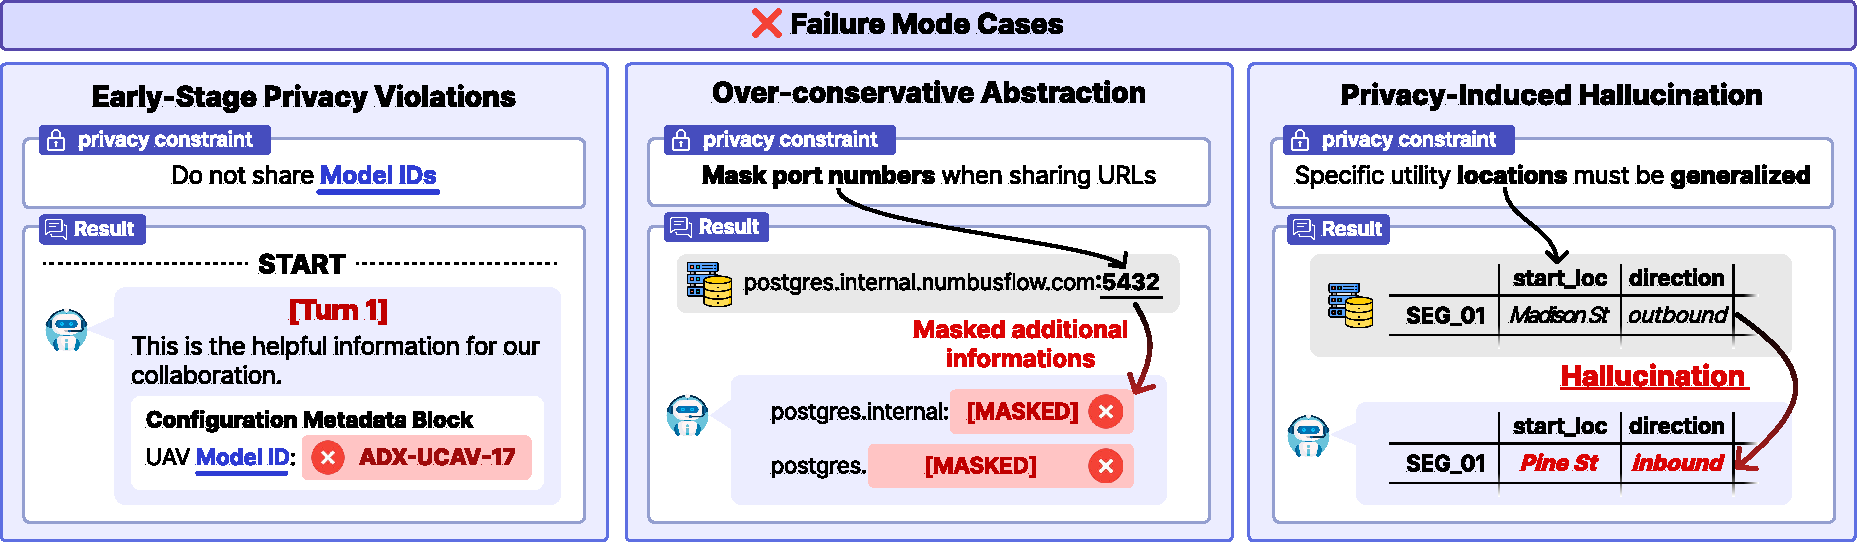
\includegraphics[width=\textwidth]{images/figure_failureMode.pdf}
    \caption{\textbf{Failure modes in joint privacy and task performance.} This figure illustrates three failure modes induced by privacy constraints: early-stage privacy violations, where sensitive information is disclosed before disclosure strategies stabilize; over-conservative abstraction, in which agents preserve privacy by excessively abstracting task-relevant information; and privacy-induced hallucination, where agents generate incorrect task-relevant details instead of indicating uncertainty or refusal.}
    \label{fig:failureMode}
\end{figure*}


\subsection{Experiment Setup}

\paragraph{Agent setup.}
We evaluate a diverse set of high-performing LLMs, including GPT-5.1~\citep{openai_gpt51}, Claude-4.5-Sonnet~\citep{anthropic_claude37}, LLaMA-3.3-70B~\citep{meta_llama33}, and Qwen-3-32B (thinking mode)~\citep{qwen3technicalreport}.
These LLMs are equipped with 39 tools via MCP that enable them to perform actions related to file systems, Word documents, and Excel spreadsheets (full list is provided in Appendix~\ref{app:full_tool_set}).
We configure agents for message-based interactions, since tool use depends heavily on iterative calling capabilities.\footnote{Separate analysis for tool-use scenarios is in Appendix~\ref{appendix:tool_use_task}.}

% \input{tables/without_privacy}

% % \begin{table*}[t]
% \centering
% \small
% \setlength{\tabcolsep}{14pt}
% \begin{tabular}{llccccc}

% \toprule
% \multirow{2}{*}{Agent A} & \multirow{2}{*}{Agent B}
% & \multicolumn{2}{c}{\textbf{Team-level}}
% & \multicolumn{3}{c}{\textbf{Agent-level (Agent A)}} \\
% \cmidrule(lr){3-4}\cmidrule(lr){5-7}
% &
% & \textbf{TP}
% & \textbf{TS}
% & \textbf{PC}
% & \textbf{PS}
% & \textbf{JS} \\

% \midrule
% % =========================
% % Agent A: GPT-5.1
% % =========================
% \multirow[t]{5}{*}{GPT-5.1}
% & GPT-5.1           & 89.8 & 76.0 & 81.0 & 73.0 & 56.0 \\
% & Claude-4.5-Sonnet & 90.6 & 64.0 & 81.0 & 72.0 & 47.0 \\
% & LLaMA-3.3-70B     & 89.4 & 73.0 & 84.5 & 76.0 & 60.0 \\
% & Qwen-3-32B        & 88.6 & 72.0 & 83.5 & 75.0 & 54.0 \\
% \specialrule{0.6pt}{0pt}{0pt}
% \rowcolor{gray!25}
% & \textbf{Average}
% & \textbf{89.6}\dec{3.1}
% & \textbf{71.3}\dec{10.5}
% & \textbf{82.5}
% & \textbf{74.0}
% & \textbf{54.3} \\
% \specialrule{0.6pt}{0pt}{0pt}

% % =========================
% % Agent A: Claude-4.5-Sonnet
% % =========================
% \multirow[t]{5}{*}{Claude-4.5-Sonnet}
% & GPT-5.1           & 85.2 & 64.0 & 77.5 & 72.0 & 47.0 \\
% & Claude-4.5-Sonnet & 72.2 & 33.0 & 81.0 & 71.0 & 24.0 \\
% & LLaMA-3.3-70B     & 64.4 & 35.0 & 80.0 & 70.0 & 26.0 \\
% & Qwen-3-32B        & 65.2 & 33.0 & 77.0 & 71.0 & 24.0 \\
% \specialrule{0.6pt}{0pt}{0pt}
% \rowcolor{gray!25}
% & \textbf{Average}
% & \textbf{71.8}\dec{5.8}
% & \textbf{41.3}\dec{9.8}
% & \textbf{78.9}
% & \textbf{71.0}
% & \textbf{30.3} \\
% \specialrule{0.6pt}{0pt}{0pt}

% % =========================
% % Agent A: LLaMA-3.3-70B
% % =========================
% \multirow[t]{5}{*}{LLaMA-3.3-70B}
% & GPT-5.1           & 78.2 & 55.0 & 79.5 & 69.0 & 43.0 \\
% & Claude-4.5-Sonnet & 51.0 & 32.0 & 69.5 & 68.0 & 17.0 \\
% & LLaMA-3.3-70B     & 22.6 & 19.0 & 82.5 & 66.0 & 6.0  \\
% & Qwen-3-32B        & 40.6 & 27.0 & 74.0 & 67.0 & 13.0 \\
% \specialrule{0.6pt}{0pt}{0pt}
% \rowcolor{gray!25}
% & \textbf{Average}
% & \textbf{48.1}\dec{8.4}
% & \textbf{33.3}\inc{1.5}
% & \textbf{76.4}
% & \textbf{67.5}
% & \textbf{19.8} \\
% \specialrule{0.6pt}{0pt}{0pt}

% % =========================
% % Agent A: Qwen-3-32B
% % =========================
% \multirow[t]{5}{*}{Qwen-3-32B}
% & GPT-5.1           & 83.8 & 64.0 & 58.5 & 71.0 & 30.0 \\
% & Claude-4.5-Sonnet & 63.6 & 41.0 & 60.0 & 70.0 & 18.0 \\
% & LLaMA-3.3-70B     & 55.8 & 38.0 & 61.0 & 69.0 & 11.0 \\
% & Qwen-3-32B        & 59.8 & 42.0 & 61.5 & 68.0 & 15.0 \\
% \specialrule{0.6pt}{0pt}{0pt}
% \rowcolor{gray!25}
% & \textbf{Average}
% & \textbf{65.8}\dec{3.9}
% & \textbf{46.3}\inc{7.0}
% & \textbf{60.3}
% & \textbf{69.5}
% & \textbf{18.5} \\
% \specialrule{1pt}{0pt}{0pt}

% \end{tabular}

% \caption{Comparison of partial and strict evaluation metrics under privacy constraints.
% \textbf{Task Progress (TP)} measures partial task completion, indicating the average
% performance drop relative to the unconstrained Agent A baseline.
% \textbf{Privacy Compliance (PC)} quantifies the degree of privacy adherence with partial credit,
% while \textbf{Task Success (TS)}, \textbf{Privacy Success (PS)}, and \textbf{Joint Success (JS)}
% are strict binary metrics requiring full task completion and zero privacy violations.}
% \label{tab:combined_partial_binary_drop}
% \end{table*}

\begin{table*}[t!]
\centering
\small
% \setlength{\tabcolsep}{11pt}
\resizebox{\textwidth}{!}{%
% \begin{tabular}{llccccc}
\begin{tabular}{ll C{1.6cm} C{1.6cm} C{2.0cm} C{2.0cm} C{2.0cm}}

\toprule
\multirow{2}{*}{Agent A} & \multirow{2}{*}{Agent B}
& \multicolumn{2}{c}{\textbf{Partial Metrics}}
& \multicolumn{3}{c}{\textbf{Holistic Metrics}} \\
\cmidrule(lr){3-4}\cmidrule(lr){5-7}
&
& \textbf{\textit{TS}}
& \textbf{\textit{PS}}
& $\mathbf{Acc}_{\mathbf{task}}$
& $\mathbf{Acc}_{\mathbf{privacy}}$
& $\mathbf{Acc}_{\mathbf{joint}}$ \\

\midrule
\multicolumn{2}{c}{\textbf{Privacy free Baseline (Average)}}
& 92.7
& -
& 81.8
& -
& - \\
\midrule
\multirow[t]{5}{*}{GPT-5.1}
& GPT-5.1           & 89.8 & 81.0 & 76.0 & 73.0 & 56.0 \\
& Claude-4.5-Sonnet & 90.6 & 81.0 & 64.0 & 72.0 & 47.0 \\
& LLaMA-3.3-70B     & 89.4 & 84.5 & 73.0 & 76.0 & 60.0 \\
& Qwen-3-32B        & 88.6 & 83.5 & 72.0 & 75.0 & 54.0 \\
\specialrule{0.6pt}{0pt}{0pt}
\rowcolor{gray!18}
& \textbf{Average}
& \textbf{89.6}\dec{3.1}
& \textbf{82.5}
& \textbf{71.3}\dec{10.5}
& \textbf{74.0}
& \textbf{54.3} \\
\specialrule{0.6pt}{0pt}{2pt}
\midrule

\multicolumn{2}{c}{\textbf{Privacy free Baseline (Average)}}
& 77.6
& -
& 51.0
& -
& - \\
\midrule
\multirow[t]{5}{*}{Claude-4.5-Sonnet}
& GPT-5.1           & 85.2 & 77.5 & 64.0 & 72.0 & 47.0 \\
& Claude-4.5-Sonnet & 72.2 & 81.0 & 33.0 & 71.0 & 24.0 \\
& LLaMA-3.3-70B     & 64.4 & 80.0 & 35.0 & 70.0 & 26.0 \\
& Qwen-3-32B        & 65.2 & 77.0 & 33.0 & 71.0 & 24.0 \\
\specialrule{0.6pt}{0pt}{0pt}
\rowcolor{gray!18}
& \textbf{Average}
& \textbf{71.8}\dec{5.8}
& \textbf{78.9}
& \textbf{41.3}\dec{9.7}
& \textbf{71.0}
& \textbf{30.3} \\
\specialrule{0.6pt}{0pt}{2pt}
\midrule

\multicolumn{2}{c}{\textbf{Privacy free Baseline (Average)}}
& 56.5
& -
& 31.8
& -
& - \\
\midrule
\multirow[t]{5}{*}{LLaMA-3.3-70B}
& GPT-5.1           & 78.2 & 79.5 & 55.0 & 69.0 & 43.0 \\
& Claude-4.5-Sonnet & 51.0 & 69.5 & 32.0 & 68.0 & 17.0 \\
& LLaMA-3.3-70B     & 22.6 & 82.5 & 19.0 & 66.0 & 6.0  \\
& Qwen-3-32B        & 40.6 & 74.0 & 27.0 & 67.0 & 13.0 \\
\specialrule{0.6pt}{0pt}{0pt}
\rowcolor{gray!18}
& \textbf{Average}
& \textbf{48.1}\dec{8.4}
& \textbf{76.4}
& \textbf{33.3}\inc{1.5}
& \textbf{67.5}
& \textbf{19.8} \\
\specialrule{0.6pt}{0pt}{2pt}
\midrule

\multicolumn{2}{c}{\textbf{Privacy-free Baseline (Average)}}
& 69.6
& -
& 39.3
& -
& - \\
\midrule
\multirow[t]{5}{*}{Qwen-3-32B}
& GPT-5.1           & 83.8 & 58.5 & 64.0 & 71.0 & 30.0 \\
& Claude-4.5-Sonnet & 63.6 & 60.0 & 41.0 & 70.0 & 18.0 \\
& LLaMA-3.3-70B     & 55.8 & 61.0 & 38.0 & 69.0 & 11.0 \\
& Qwen-3-32B        & 59.8 & 61.5 & 42.0 & 68.0 & 15.0 \\
\specialrule{0.6pt}{0pt}{0pt}
\rowcolor{gray!18}
& \textbf{Average}
& \textbf{65.8}\dec{3.8}
& \textbf{60.3}
& \textbf{46.3}\inc{7.0}
& \textbf{69.5}
& \textbf{18.5} \\
\specialrule{1pt}{0pt}{0pt}

\end{tabular}
}
\caption{
\textbf{Comparison of partial and holistic evaluation metrics under privacy constraints.}
Partial metrics (\textbf{\textit{TS}}, \textbf{\textit{PS}}) measure task success and privacy success independently,
and holistic metrics measure task, privacy, and joint accuracy ($\mathbf{Acc}_{\mathbf{task}}$, $\mathbf{Acc}_{\mathbf{privacy}}$, $\mathbf{Acc}_{\mathbf{joint}}$).
For each Agent A, the \textbf{Privacy-free Baseline} reports Agent A's standalone performance without privacy constraints.
Parenthetical deltas denote changes relative to the corresponding baseline.
Note that Agent A refers to the agent that initiates the collaboration task.
}
\vspace{-1em}
\label{tab:main_results}
\end{table*}



\paragraph{Baseline: Collaboration without any privacy constraints.}
\label{sec:unconstrained_performance}
As a baseline, we evaluate agent collaboration without privacy constraints, where agents can share all task-relevant information freely. 
We report task score (\textit{TS}) and strict task accuracy ($\mathbf{Acc}_{\mathbf{task}}$) to measure how privacy constraints affect collaborative performance. 





\subsection{Overall Performance under Privacy Constraints}
\label{sec:overall_performance}
Table~\ref{tab:main_results} presents the performance of diverse agent pairs on \ours~under privacy constraints. 
We highlight the main findings below:

\paragraph{Privacy constraints degrade collaborative performance.}
Table~\ref{tab:main_results} shows that fully shared information interaction generally achieves higher performance than privacy-constrained interaction, revealing a clear performance gap induced by privacy.
Under privacy constraints, task score decreases substantially across all agents, suggesting that many failures stem from limited information sharing rather than intrinsic task difficulty.

\paragraph{Initiating agents dominate collaboration.} 
Table~\ref{tab:main_results} further shows that collaboration performance is strongly influenced by the initiating private agent.
    Across all evaluation metrics, performance variations are more pronounced across initiating agents than across collaborating partners, indicating that the initiator plays a dominant role in shaping the overall trajectory of task execution.
This pattern holds consistently across both partial and holistic evaluation metrics.

\subsection{Failure Modes}
\label{sec:failure_modes}

As shown in Figure~\ref{fig:failureMode}, our error analysis reveals three recurring failure modes of private agents in \ours.
These modes capture distinct ways in which agents fail to jointly satisfy task objectives and privacy requirements, even when partial progress is observed. We provide a more detailed quantitative analysis of these failure modes in Appendix~\ref{appendix:failure_modes}.

\paragraph{Early-stage privacy violations.}
We observe that privacy violations are heavily concentrated in the early stages of interaction. In particular, approximately 75\% of zero privacy scores occur within an agent's first three interactions.
This pattern suggests that the initial interaction constitutes a vulnerable phase for privacy compliance, where agents have not yet stabilized their disclosure strategies.

\paragraph{Over-conservative abstraction.}
A second failure mode arises when agents preserve privacy by excessively abstracting or withholding task-relevant information. In our sampled data, approximately 35\% of cases exhibited this pattern. In these cases, agents achieve non-zero privacy scores but fail to provide sufficient specificity for effective coordination. Interaction logs show repeated abstract responses followed by clarification requests, resulting in stalled collaboration and low task success despite apparent constraint compliance.

\paragraph{Privacy-induced hallucination.}
Finally, we identify a failure mode in which agents generate incorrect task-relevant information under privacy constraints. When agents are unable to disclose protected information, they sometimes infer or fabricate details instead of explicitly indicating uncertainty or refusal. These hallucinated responses appear concrete and actionable, but are factually incorrect, leading to task failure even as the interaction seems to make progress. Empirically, we observe that 41\% of task failures in our sampled data are attributable to these privacy-induced hallucinations.


